\chapter{Business Model for the Kinect Based Exercise Game}
\section{Product}
A product covers all aspects of what a company offers to its customers. The product is composed of value propositions, which are services and values offered to the customer. Cyberlab will develop an exercise game used by physiotherapists in prevention and rehabilitation for elderly. The focus of the exercise game is to improve strength and balance in elderly to prevent fall and injuries. The idea is that this game should have one general workout version directed towards prevention and one more customized version used in rehabilitation.
\subsection{Value Proposition}
Value propositions refer to the value a company offers to a specific customer segment. One of the values this product gives to the customer is an opportunity to offer an alternative, fun and motivation training method. The exercise game could be used as a supplement in training programs or as an exercise motivator. A good motivator is a social aspect, which is highly important for elderly, and that there exist games for different interests. The game could also be used as a tool for physiotherapists to make it easier to customize training programs for their patients. Every patient is different, with individual problems and needs, and it is therefore necessary to provide personalized exercise program for each patient. An important value the product has to serve is that the exercise game can set up training programs and be more motivating than a physiotherapist can. To get a consultation hour at a physiotherapist there is often long waiting lists, so it is important for the physiotherapists to be efficient to serve as many patients as possible, without losing quality in the work done. By using this exercise game it is possible to ease the physiotherapists’ workload. The ability of this game is that it can serve more than one player at the same time, which means that a physiotherapist can consult and exercise with more patients in one hour than a physiotherapist can manage without the exercise game. This would be a helpful in the work of shortening the long waiting lists.
\section{Customer Interface}
In this section we will describe how Cyberlab can create value to the customers. Who are the customers, how will they establish contact with them and how will they maintain customer relationship after sales.
\subsection{Customer Segments}
In general, a company generates value for a specific customer segment. The target customer for Cyberlab in this business model is physiotherapists working in both local and private institutes.  This is an entity that has a very close relationship with elderly. A goal for a physiotherapist is to help elderly decrease the risk of falling by using mobility techniques to improve balance and physical strength. One thing to pay attention to is that customers not always are the end user, and that it is important to recognize this difference. A satisfied end user is important for the customer, although they are not the same person. In the beginning we were thinking about elderly as a target customer segment for Cyberlab as they are the end users of the product. After working with and studied this business model we experienced that elderly is not the right target for Cyberlab after all. There are some reasons for that. Elderly today doesn’t have a relation to the type of technology Cyberlab is trying to sell, so it would be very difficult to reach out to this customer segment. So how can Cyberlab reach its end users?  One solution would be to go through someone elderly can trust and rely on. Elderly, as almost everyone else, relies on authorities, and physiotherapists are an example of that kind of authority.  
\subsection{Channels}
This subsection about distribution channels describes how Cyberlab should deliver and market their value propositions to the customers. We will describe this by going through the five channel phases.\\ \\
\begin{figure}[h]
\caption[Channels]{The 5 Channel Phases [modified from \cite{osterwalder} \cite{osterwalderthesis}]}
\label{fig:Channels}
\begin{center}
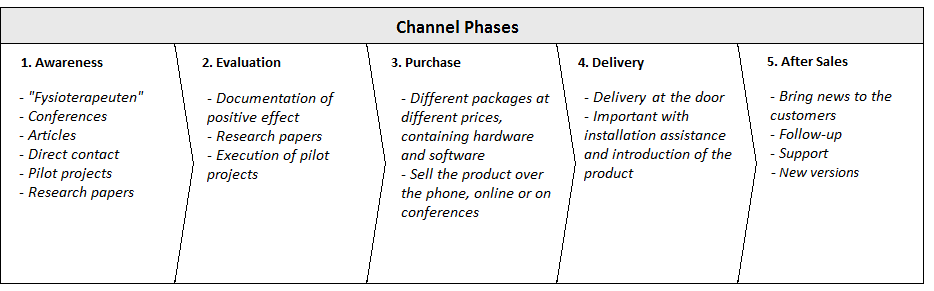
\includegraphics[scale=0.7]{channels}
\end{center}
\end{figure}
\emph{Awareness:} \\ 
We will look into how Cyberlab can raise awareness about the product and how they can get their customers attention.  “Fysioterapauten” is a magazine targeting physiotherapists in Norway. It is published by NFF (Norsk Fysioterapeutforbund) and distributed out to the whole country. “Fysioterapauten” contains mostly scientific papers, and the idea is that this magazine shall contribute to evolvement of the physiotherapy profession according to the society and populations need. This magazine is read by 9 000 physiotherapists around the country, and articles printed here are seen as scientific and are therefore taken seriously.  If Cyberlab could get an article or ad in “Fysioterapauten” it will contribute to great exposure of the exercise game.  Printing research papers and articles about the exercise game in other credible magazines or newspapers could also get physiotherapists attention.  Taking direct contact with target customers is also a possible solution. This could be done on conferences related to the subject of e.g. technology and health or by visiting physiotherapy institutes. Cyberlab could get the opportunity to present the products and show direct interest in establishing a customer relationship. Physiotherapists see it as very relevant to try a product for an amount of time before they decide to buy. By taking direct contact Cyberlab can introduce a pilot project to the customer, which means testing the product for free in e.g. 6 months. Through conferences, magazines or just word of mouth one can also get an impression of which products that are popular right now. The popularity mark might attract some customers. Physiotherapists working at private institutes don’t have the same access to customers as local institutes have, so they might chose to buy a popular product to attract new and more customers. (vet ikke om dette passer under her..)\\ \\ 
 (Nav- hjelpemiddelsentralen)\\ \\
\emph{Evaluation:}\\
Physiotherapists points out two very important aspects in evaluating a product. These two are documented effect of the product and own experience by testing the product. If a physiotherapist should even think about trying the product it is necessary to provide research papers or statistics that shows positive effect in this kind of games. Documentation will give them a security in the choice of buying the product. (Merkelig setning??) Other physiotherapists providing positive feedback after trying the game also contributes to this security. Another part of the evaluation is by letting physiotherapist be part of pilot projects for a period of time. Then they can test the product and experience themselves if the product works or not.\\ \\
\emph{Purchase:} \\
Several physiotherapists give the impression that they already have established connections with suppliers. Ordering and buying products are usually done online, but it can also be by phone or when interesting products are discovered on conferences. Going to the store to buy products are very unusual. But what will physiotherapists buy from Cyberlab? To play this game you need an Xbox Kinect and the exercise game. It is unreasonable to think that a physiotherapist already owns an Xbox Kinect, so the best thing for Cyberlab would be to sell packages containing both hardware and software.  Packages should include various agreements with appropriate pricing. Some examples are selling the package with or without installation assistance and introduction to the product, or by selling a license agreement and “give away” the package for free.\\ \\
\emph{Delivery:}\\
 When buying a new product, especially technical products, there is a need for introduction to the product and maybe also installation assistance. Feedback from interviews with physiotherapists shows the huge importance of startup help. With much to do at work already, physiotherapists don’t have time to pick up deliveries at the postal office, or to setup and learn a new product all by themselves. Buying, receiving, installing and learning should not be difficult or time consuming. The product should be delivered at the door, by someone who can install the product and teach the physiotherapists how to use it.\\ \\
\emph{After sales:}\\
When taking a new product in to use, it is important for physiotherapist to have the possibility to provide feedback. Therefore, Cyberlab should have some kind of support that can take these feedbacks into consideration. Feedbacks can be comments on direct errors or directions on how to make the exercise game more suitable for its use. Cyberlab should follow their customer in the process of learning, and they should inform them of new features and improvements.  
\subsection{Customer Relationships}
Customer relationship is an important part of the customer experience, and it describes what kind of relationship the company establishes with the customers. Support, follow-up and feedback handling are some aspects in establishing customer relationship. Cyberlab has to be available when the customers has problems and needs help. When using a new product one may discover errors or find the product not suitable for its use, so many physiotherapists have an eager to provide feedback on this. Cyberlab should handle these feedbacks, fixe errors as soon as possible and take comments on improvements into consideration. Using feedback to make a better product shows customers that Cyberlab takes their comments seriously.  In addition, the customers will hopefully get a more suitable product. The maintenance of a direct and personal contact with the customer shows interest in the use and the experience of the product. All this can contribute to a good customer relationship. Cyberlab should also give their customers a heads ups on updates, new features or products.
\section{Infrastructure Management}
This section is about how Cyberlab creates value. What resources needed and what activities that have to be preformed are described here, as well as if they will get them in-house or from a partner. 

\subsection{Key Resources}

In this section we will describe all the resources needed to make the business model work. The resources are divided into 4 different types, described in table \ref{tab:Resources}.
\newpage

\begin{table}
\centering
    \begin{tabular}{|l|l|}
        \hline
       \textbf{Type of Resource} & \textbf{Resource}  \\ \hline
       \emph{Intellectual} & Insight and experience with fall problematic in elderly \\ \cline{2-2}
        & Programming skills \\ \cline{2-2}
	 	& Creativity \\ \hline
	   \emph{Physical} & Premises \\ \cline{2-2}
	   	& Equipments, i.e. desks and computers \\ \cline{2-2}
	   	& Microsoft Xbox HW \\ \cline{2-2}
	   	& Working Environment \\ \cline{2-2}
	   	& Internet Connections \\ \hline
	   \emph{Human} & System Developers, i.e. programmers and interaction designers \\ \cline{2-2}
	   	& Administration, i.e. marketers, customer related tasks \\ \cline{2-2}
	   	& Support Person(s) \\ \hline
	   \emph{Financial} & The European Union \\
        \hline
    \end{tabular}
    \caption[Resources]{Different types of resources}
    \label{tab:Resources}
\end{table} 
\emph{Intellectual} \\ The developers needs insight and knowledge about different exercises that will strengthen muscles and improve balance in elderly. A thorough background study and research have to been conducted to acquire this knowledge. When they have enough knowledge to form the foundation of an exercise program, they can start to get creative. Creativity is needed to make the game entertaining and east to understand and conduct. In addition to that, good programming competencies is needed to develop the game. To make it as cost-efficient as possible, an experienced team should be put together. \\ \\
\emph{Physical} \\ To be able to conduct this project, the team need premises with everything that comes with it, like desks, chairs, computer, internet connection, light etc. Cyberlab is an already established business, so we can assume they already have these premises and equipments established. For this project, they will need specific hardware. The hardware consists of Xbox 360 console and Kinect sensor. In addition an environment where the game can be developed is needed. \\ \\
\emph{Human} \\ Programming skills and creativity are already described above as intellectual resources. So system developers and interaction designers are needed. An administration is needed for marketing, customer related tasks and resource management. When the game is finished it needs to be operated and maintained. These tasks can be done by one or more of the system developers. \\ \\
\emph{Finance} \\ This project is financed by the European Union. 
\subsection{Key Activities}
The game can be described as Value Chain, which means transforming inputs to a final product. From the knowledge and experience they have acquired the company wants to make a product as good and price-competitive so that their customers would choose their product instead of a product with similar value. A description of the different stages in the value chain is depicted in figure \ref{fig:ValueChainCase}. In some way it can also be thought of as kind of a Value Shop, because they are in some way solving a problem for a specific customer segment. To do this, they will work in an iterative way, where they will have to test and evaluate the game during the development process. The users have to be involved during the development. 
Activities that need to be done include research, development, testing, maintenance and updates, support, marketing and administrative tasks. 
\begin{figure}[h]
\caption[ValueChainCase]{Value chain for the Kinect based game [modified from \cite{osterwalderthesis}]}
\label{fig:ValueChainCase}
\begin{center}
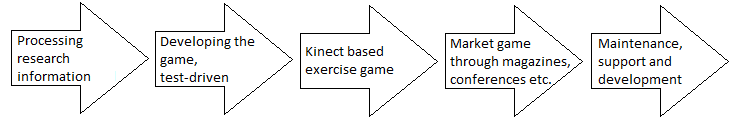
\includegraphics[scale=0.7]{valuechaincase}
\end{center}
\end{figure}
\subsection{Key Partnerships}
The main partner in this project is the partnership with the Microsoft Xbox. There are several reasons for this. First of all, they need the approvement that they are allowed to develop games for their video game console, and second, they need Microsoft Xbox’ hardware and development environment. They will also have to form an agreement with Microsoft Xbox on how they can sell the product. \\ \\ As mentioned in the introduction, this project is a collaboration between many different entities, where Norut, a national research group, is one of them. Their job in this project is to provide Cyberlab with …... finne ut av dette........ \\ \\ Physiotherapists are their customer segment, but they can also serve as a partner. Becoming partners with different clinics, will make the the marketing and selling easier, because then the actual customer believes in it. \\ \\ If professionals, physiotherapists believes in this, then the government should believe in it. Getting this game into a medical program financed by the government will make this game very credible for the end user. The Government could then provide the game to hospitals, care centers, physiotherapy clinics, training groups, and for special cases, when the elderly for example stays in their own house. \\ \\ Becoming partners with the Norwegian Government will first require that the physiotherapists believes in it, so they will first have to join the team. But it is not a requirement that physiotherapists become a partner. But some kind of collaboration has to be established with the physiotherapists. This will typically happen in the research, - development -and testing phase. \\ \\ Having the Norwegian Government as a partner will solve some of the financial issues. Most hospitals, physiotherapy clinics and training groups are managed and financed by the Government. With them believing in the game and including it as a helping tool that will prolong and improve elder's life it will be easier to hit the target users. 
\section{Financial Aspects}
In this section all the outgoing and incoming money will be described. All the previous blocks described are contributing to a cost or an income. We will try to provide an as realistic and detailed estimate of both costs and income.
\subsection{Revenue Streams}
The revenue stream describes how the company can earn money, and for Cyberlab this involves selling a product package consisting of the Xbox Kinect and the exercise game. There are various ways to sell this product, and we will describe three possibilities. First, the easiest solution is to sell only the package and let the customers install and learn the product themselves. A second solution is to sell the package with delivery, install assistance and introduction of the product. We have experienced that this is an interesting alternative for physiotherapists. This second solution will also, more than the first alternative, contribute to establishment of customer relationship (KAN JEG SI DETTE??). The third solution is selling the package implemented in a license agreement. Customers will not pay directly for the package, but they will pay a certain amount of money for the time they use the product. This license solution can if needed be sold with or without the delivery and installation assistance. Ilen Fysioterapi og Idrett, a private physiotherapy institute sees a security in the possibility of buying the product with a license agreement. They might not have the same financial resources as local institutes, so the idea of paying according to how much they use the product is appealing. Through interviews we have experienced that most physiotherapy institutes buy products instead of renting. Renting usually happens when one local physiotherapy institute owns a product another local institute might need.
\begin{table}
\centering
    \begin{tabular}{|l|l|}
        \hline
       \textbf{Package example} & \textbf{Price example}  \\ \hline
       Only the package & 4 000 NOK \\ \hline
	   Package with delivery, installation and introduction & 8 000 NOK \\ \hline
	   Package as a license agreement & 9 500 NOK\\ \hline
	   Package as a license agreement with delivery, \\ 
	   installation and introduction & 13 500 NOK \\
        \hline
    \end{tabular}
    \caption[Priceexample]{A price example}
    \label{tab:Priceexample}
\end{table} 

\subsection{Cost Structure}
Cost structure takes all elements that generates cost specific to this game into account. Cyberlab is an already established business and we can therefore assume that there are not any additional costs associated with premises and some of the “regular” equipments. First we distinguish between fixed and variable costs. In this case fixed costs are associated with salaries to the project team, which includes project manager, developers, researchers, interaction designers and marketers. We define these as fixed costs because the employers are hired to do this job over a fixed period of time. Other fixed costs include hardware and software that are needed to set up an environment for developing of the game. (Prøve å få faktiske tall fra tor ivar her..) Variable costs in this case includes Xbox hardware depending on the demand from the customers. 

